\chapter{Lecture 2: Probabilities}
Probability theory allows us to mathematically model processes governed by chance or random phenomena. As such, it provides a mathematical foundation for statistics. We can use probability theory to determine when a process, such as the random flipping of a coin, deviates from its expected behaviour, perhaps due to an \textbf{unfair} coin, or some kind of interference, like friction. Some of the less obvious modern applications of probability theory are found in cryptography, statistical mechanics, computer science, and quantum physics. \\

\noindent We do not use probability to model deterministic events, such as the time that the sun will rise in the morning; but we do use it to model chance events, like the likelihood of rain.  \\

\noindent Like many mathematical ideas (see section \ref{axioms}), probability theory rests on a small number of axioms. These axioms will be worth remembering, because they tell us when a \textbf{function} is a \textbf{probability measure}. We introduce the ideas of function and probability measure along with the axioms below.
 
\section{Functions and probability measures}
%DIRECT FROM SLIDES
\subsection{Some terminology}
We refer to questions about chance phenomena as \textbf{experiments}. The set of all possible \textbf{outcomes} of an experiment is called the \textbf{sample space} (sometimes called the \textbf{outcome space}), written $\Omega$ or $S$ \label{symbS} (this is the universal set). A single element of $\Omega$ may be written $\omega$ \label{symbomega} (this is the lower case Greek letter `omega'). Any subset of $\Omega$ is called an \textbf{event}. We usually use a capital letter (e.g. A,B, or C) to represent events; though we often define the events using words. We may refer to an object as \textbf{fair} (or \textbf{unfair}), or \textbf{balanced} (or \textbf{unbalanced}). The terms fair and balanced imply that the object behaves as expected; for example a fair coin will have a 50\% chance of landing heads and a 50\% chance of landing tails. It is worth mentioning that we still do not have a mathematical definition of this use of the word `chance.' This will soon be remedied. \label{unfair} \label{balanced} \label{experiment} \label{sample space} \label{outcome} \label{event}

\subsection{Example} \label{outcome space}
If our experiment consists of flipping a fair coin \textbf{and} rolling a balanced, standard 6-sided die, then what is the sample space? \\

Solution:
\begin{align*}
\Omega = & \{(\text{heads},1),(\text{heads},2),(\text{heads},3),(\text{heads},4),(\text{heads},5),(\text{heads},6), \\
		& \;\;(\text{tails},1),\;(\text{tails},2),\;(\text{tails},3),\;(\text{tails},4),\;(\text{tails},5),\;(\text{tails},6)\}
\end{align*}

\noindent Let $A$ be the event that we roll a 6. Describe $A$ as a subset of the sample space. \\

Solution:
\[
A = \set{(\text{heads},6),(\text{tails},6)}
\]

%------------------------------------------------------------Page 10

\subsection{Intro to functions} \label{sectionfunctions}
A function \label{function} is a rule that assigns elements of one set to elements of another set. This assignment is sometimes called ``\textbf{mapping}.'' We may, for example, have the set $\set{2,5,7}$ and we might create a function that assigns an element from $\set{\text{red},\text{yellow},\text{blue}}$ to each element from $\set{2,5,7}$. \label{mapping}. We say that the function ``maps $\set{2,5,7}$ to $\set{\text{red},\text{yellow},\text{blue}}$.'' We can visualise functions using arrow diagrams as follows:
\begin{center}
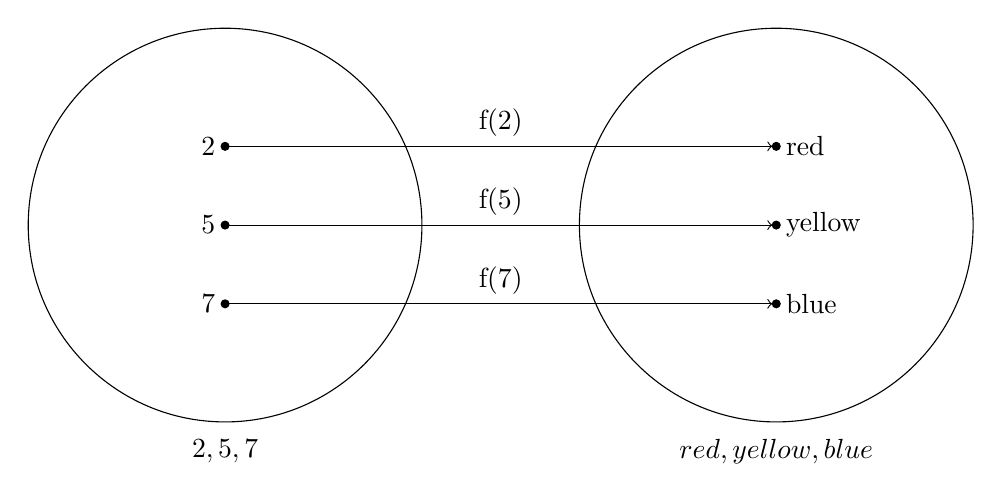
\begin{tikzpicture}
	\draw (0,0) circle (2.5cm) node [below = 2.6cm] {$\set{2,5,7}$};
	\draw (7,0) circle (2.5cm) node [below = 2.6cm] {$\set{\text{red,yellow,blue}}$};
	\draw [->] (0,0) -- (7-0.05,0);
	\draw [->] (0,1) -- (7-0.05,1);
	\draw [->] (0,-1) -- (7-0.05,-1);
	\draw [fill = black] (0,1) circle (0.05cm) node [left] {$2$};
	\draw [fill = black] (0,0) circle (0.05cm) node [left] {$5$};
	\draw [fill = black] (0,-1) circle (0.05cm) node [left] {$7$};
	\draw [fill = black] (7,1) circle (0.05cm) node [right] {red};
	\draw [fill = black] (7,0) circle (0.05cm) node [right] {yellow};
	\draw [fill = black] (7,-1) circle (0.05cm) node [right] {blue};
	\draw (3.5,1) node [above] {f(2)};
	\draw (3.5,0) node [above] {f(5)};
	\draw (3.5,-1) node [above] {f(7)};
\end{tikzpicture}
\end{center}

\noindent In the above diagram our function is the rule: map~2~to `red,' map 5 to `yellow,' and map 7 to `blue.' We have called this function~$f$, so we write
\[
f(2) = \text{`red,'} \qquad f(5) = \text{`yellow,'} \qquad f(7) = \text{`blue.'}
\]
For convenience we can define~$X~=~\set{2,5,7}$ and $Y = \set{\text{red},\text{yellow},\text{blue}}$. Then $f$ is a function from $X$ to $Y$. \\

\noindent A function does not need to map to all of the elements in $Y$. We could have, for example, a function (say $g$) that has the rule 
\[
g(2) = \text{`red,'} \qquad g(5) = \text{`red,'} \qquad g(7) =  \text{'red.'} 
\]
On an arrow diagram, $g$ appears as follows:
\begin{center}
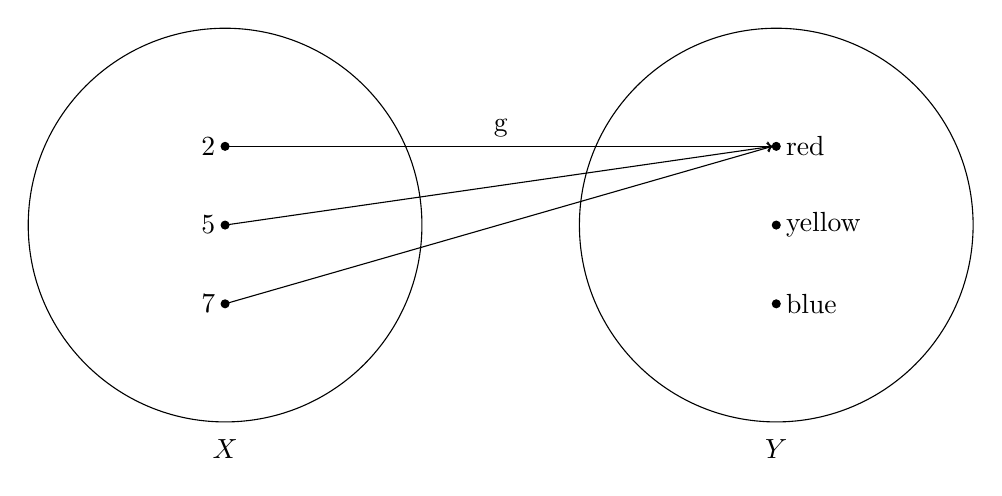
\begin{tikzpicture}
	\draw (0,0) circle (2.5cm) node [below = 2.6cm] {$X$};
	\draw (7,0) circle (2.5cm) node [below = 2.6cm] {$Y$};
	\draw [->] (0,0) -- (7-0.05,1);
	\draw [->] (0,1) -- (7-0.05,1);
	\draw [->] (0,-1) -- (7-0.05,1);
	\draw [fill = black] (0,1) circle (0.05cm) node [left] {$2$};
	\draw [fill = black] (0,0) circle (0.05cm) node [left] {$5$};
	\draw [fill = black] (0,-1) circle (0.05cm) node [left] {$7$};
	\draw [fill = black] (7,1) circle (0.05cm) node [right] {red};
	\draw [fill = black] (7,0) circle (0.05cm) node [right] {yellow};
	\draw [fill = black] (7,-1) circle (0.05cm) node [right] {blue};
	\draw (3.5,1) node [above] {g};
\end{tikzpicture}
\end{center}

\noindent We can still say that $g$ is a function from $X$ to $Y$; we do not require that every element in $y$ is a possible output of $g$. However, \textbf{we always choose $X$ so that our function assigns something to every element in $X$} (unlike the case with $Y$). This asymmetry with our conditions for $Y$ and our conditions for $X$ may seem strange at first but this is an important part of the definition of a function. \\

\noindent When a function maps from a set $X$ to a set $Y$, we call $X$ the \textbf{domain} \label{domain} of the function, and we call $Y$ the \textbf{codomain}. The set of all possible outputs of the function are called its \textbf{range}. \\

\noindent The range of $g$ is the set $\set{\text{red}}$, while its codomain is still $Y$. On the other hand, the range of $f$ is $Y$, and the codomain of $f$ is also $Y$, because $f$ maps to every element in $Y$. \\

\noindent It is clear from our descriptions of ``range'' and ``codomain'' that the range of a function must always be some subset of the codomain (or equal to the codomain). In general, an arrow diagram of some arbitrary function, $h$, can be drawn as follows:
\begin{center}
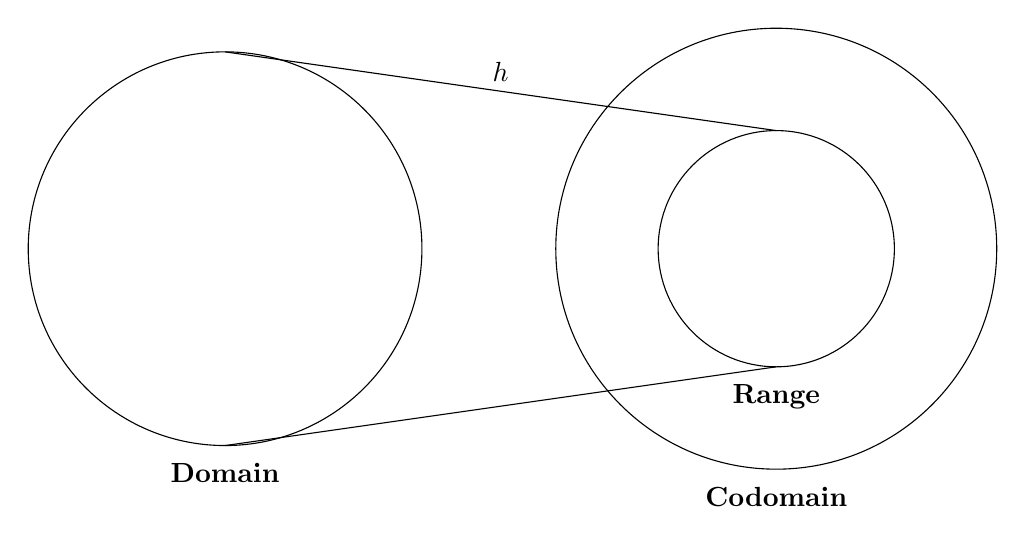
\begin{tikzpicture}
	\draw (0,0) circle (2.5cm) node [below = 2.6cm] {\textbf{Domain}};
	\draw (7,0) circle (2.8cm) node [below = 2.9cm] {\textbf{Codomain}};
	\draw (7,0) circle (1.5cm) node [below = 1.6cm] {\textbf{Range}};
	\draw (0,2.5) -- (7,1.5);
	\draw (0,-2.5) -- (7,-1.5);
	\draw (3.5,2) node [above] {$h$};
%	\draw [->] (0,0) -- (7-0.1,0);
%	\draw [fill=black] (0,0) circle (0.05cm);
%	\draw [fill=black] (7,0) circle (0.05cm);
\end{tikzpicture}
\end{center}
\noindent This diagram is intended to indicate that every element from the domain is mapped to some element from the range, and that every element from the range has something mapped to it. The diagram also indicates that, unlike the range, the codomain may have elements that are not mapped to at all by $h$.

\noindent The functions that we deal with in probability will mostly be functions that map from subsets of $\Omega$ to $\R$. Hence their range will be some subset of $\R.$ We will see below that this is one of the conditions for a function to be called a probability measure.  \label{range} \label{codomain}

\subsection{Probability measure axioms} \label{paxioms}
%MORE OR LESS OUT OF THE SLIDES LECTURE 2
An \textbf{axiom} is a certain condition or rule that is placed on a mathematical idea. As stated in section \ref{axioms}, in some sense the goal of mathematics is to formulate a set of rules or conditions (axioms) and then to just find out what the logical consequences of those rules are. Here we introduce the axioms that all of the mathematical ideas in probability rest on; the probabilty measure axioms. A probability measure \label{probability measure} is a function, we will label it $P$, that maps subsets of $\Omega$ (called events) to $\R$, and satisfies the following three basic axioms \label{symbP()} \label{axiom}
\begin{enumerate}
\item $P(\Omega) = 1$
\item For any event $A \subseteq \Omega,$ we have $P(A) \geq 0$
\item If two events $A$ and $B$ are disjoint, then $P(A \cup B) = P(A) + P(B)$
\end{enumerate}
It is remarkable that there are only three simple axioms. You will get plenty of practice with these three axioms so don't worry if they look a little confusing now. \\

\noindent Probability measures are functions that we use to express the likelihood of an event. We will soon see (in section \ref{consequences}) that, as a consequence of the axioms, the probability of any event is a number between 0 and 1. For any two events $A,B$ we say that, if $P(B) = 0$, then $B$ is impossible. If $P(A) = 1$ then we interpret this to mean that $A$ will definitely occur. If $P(A) > P(B),$ then $A$ is more likely than $B$; we read this as saying ``the probability of $A$ is greater than the probability of $B$''. You can read the statement $P(A) = x$ for any number $x$ as \textit{``the probability of $A$ occurring equals $x.$''}

\subsection{Example}
Consider axiom 3. Suppose that on any given day we suspect that 70\% of people listen to music at home, and 50\% of people listen to music at work; then does this imply that 120\% of people listen to music at some time during the day? The answer is clearly no; it is not possible to have more than 100\%. The problem is that some people might listen to music both at home \textit{and} at work; this implies that the intersection of the events is non-empty (see page \pageref{disjoint}), i.e. the events are not disjoint. Hence axiom 3 is not relevant in this case.

\subsection{Consequences of probability measure axioms} \label{consequences}
As is the case with any axiomatic system, the other properties of probability measures all follow logically from the three axioms. Consider the following important consequences. In appendix \ref{appendix A} we have included proofs that these consequences follow logically from the probability measure axioms. It is a good idea to read through the proofs carefully.
\begin{itemize}
\item \textbf{Consequence 1} \label{consequence1} \\
If the events $A, B$ and $C$ are \textbf{mutually disjoint} \label{mutually disjoint} (that is, for any pair of two events, the intersect of that pair is empty), then \\
$P(A \cup B \cup C) = P(A) + P(B) + P(C)$. \\

This extends logically to more than 3 mutually disjoint events.
\item \textbf{Consequence 2} \\
For any event $A$, \\
$P(A^c) = 1 - P(A).$

\item \textbf{Consequence 3} \\
$P(\varnothing) = 0.$

\item \textbf{Consequence 4} \\
If $A \subseteq B$, then $P(A) \leq P(B)$.

\item \textbf{Consequence 5 (the Addition Law)} \label{addition law} \\ 
For any events $A$ and $B$ \\
$P(A \cup B) = P(A) + P(B) - P(A \cap B)$
\end{itemize}

\subsection{Example (consequence 4)}
%STRAIGHT OUT OF SLIDES
Let $B$ be the event that the total shown on two standard 6 sided dice is exactly 2, and let $C$ be the event that at least one of the dice shows a 1. Then 
\[
B = \set{(1,1)}, \; \text{and}\;\; C = \set{(1,1),(1,2),(1,3),(1,4),(1,5),(1,6),(2,1),(3,1),(4,1),(5,1),(6,1)}.
\]
So we can observe that $B \subseteq C$. Hence $P(B) \leq P(C)$ by consequence 4. \\

\noindent We will look deeper into the rest of consequences 1 to 5 in later sections (and in appendix A).



\section{Assigning probabilities to events}
Choosing how to assign probabilities to events in a given situation usually requires empirical evidence from experimental results. The models that we will develop during this course will all represent different ways of assigning probabilities to events. Much of the science in applied probability goes into choosing how and when to apply these models. \\

\noindent The probability measure axioms tell us nothing about how we should assign probabilities to events. As long as we are consistent with the axioms, we can choose to assign the probabilities in whatever way best suits our purposes. \\

\noindent The universal set, $\Omega$, is a collection of elements (we refer to these elements as ``outcomes'', and label them $\omega$, see page~\pageref{outcome}). If $\Omega$ is finite in size, then we can assign a probability to each outcome $\omega.$ Then, for any event $A \subseteq \Omega$, we can assign a probability to $A$ by adding together the probabilities of each outcome in $A$.
\subsection{Example} \label{example2.2.1}
%STRAIGHT OUT OF LECTURES
Let $A$ be the event that the total shown on two standard 6 sided dice is exactly 6. Let $B$ be the event that the total shown is exactly 2. Let $C$ be the event that at least one of the dice shows a 1.  Then what are the respective probabilities of $A,B$ and $C$? We have,
\begin{align*}
&A = \set{(1,5),(5,1),(2,4),(4,2),(3,3)}, \\
&B = \set{(1,1)}, \\
&C = \set{(1,1),(1,2),(1,3),(1,4),(1,5),(1,6),(2,1),(3,1),(4,1),(5,1),(6,1)}.
\end{align*}
The total number of possible outcomes from rolling two 6 sided dice is 36 (later, we will look at ways to count outcomes without listing them all, see example \ref{ex3.0.9}). It is reasonable for us to assume that if the dice are fair, then each of the 36 outcomes is equally likely. To satisfy axiom 1 we need to make sure that the sum of the probabilities of all the outcomes is 1; these considerations suggest that we assign a probability of $\frac{1}{36}$ to each outcome. \\

\noindent Since $A$ contains $5$ outcomes we get 
\[
P(A) = \frac{1}{36} + \frac{1}{36} + \frac{1}{36} + \frac{1}{36} + \frac{1}{36} = \frac{5}{36}.
\]
Similarly, since $B$ contains 1 outcome and $C$ contains 11 outcomes, so
\[
P(B) = \frac{1}{36} \qquad \text{and} \qquad P(C) = \frac{11}{36}.
\]


\subsection{Equally likely outcomes} \label{sec222}
%STRAIGHT OUT OF LECTURES
The simplest situation that we can have is a finite list of basic outcomes, each of which is equally likely. Suppose we have $N$ different outcomes, then
\begin{align*}
\Omega & = \set{\omega_1,\omega_2,\omega_3,\ldots,\omega_N} \\
	     & = \set{\omega_1} \cup \set{\omega_2} \cup \set{\omega_3} \cup \ldots \cup \set{\omega_N}.
\end{align*}
Since the individual outcomes are single elements they are disjoint so, by consequence 1
\begin{align*}
P(\Omega) = P(\set{\omega_1}) + P(\set{\omega_2}) + P(\set{\omega_3}) + \ldots + P(\set{\omega_N}).
\end{align*}
Since this is the simplest situation we can have, i.e. since each outcome is equally likely, we have $ P(\set{\omega_1}) = P(\set{\omega_2}) = P(\set{\omega_3}) = \ldots = P(\set{\omega_N})$. So if we let $\omega$ represent any arbitrary one of these outcomes, we can write
\[
P(\Omega) = N\times P(\set{\omega})
\]
To satisfy axiom 1 we require $P(\Omega) = 1$ so this means we must have $1 = N\times P(\set{\omega})$. \\ Therefore, $P(\set{\omega}) = \frac{1}{N}.$ We often just leave out the set brackets around $\omega$ by convention to simplify the notation. So \textbf{in the case of a finite universal set of $N$ equally likely outcomes} we have

  	\bigskip
	
	\hfil\fbox{
	\begin{minipage}{0.3\columnwidth}{
	
	\vskip 0.02cm
	\begin{center}
	$\displaystyle{P(\omega) = \frac{1}{N} = \frac{1}{\text{Size}(\Omega)}}$
	\end{center}
	}
	\end{minipage}}
	\bigskip
	\bigskip
	
\noindent Now, suppose we want the probability of an event, $E$, where
\[
E = \set{\omega_1,\omega_2,\ldots,\omega_m}, \qquad \text{for some $m \leq N$},
\]
and where every element in the outcome space is equally likley. Note that $m$ is equal to the number of elements in $E$, so $m = $ Size($E$). Then we just need to recognise that
\[
E = \set{\omega_1} \cup \set{\omega_2} \cup \ldots \cup \set{\omega_m},
\]
which is a union of disjoint sets, so
\begin{align*}
P(E)  & = P(\omega_1) + P(\omega_2) + \ldots + P(\omega_m) \tag{by probability measure axiom 3} \\
	& = \underbrace{\frac{1}{N} + \frac{1}{N} + \ldots + \frac{1}{N}}_{m \text{ times}} \tag{by the result in the box above} \\
	& = \frac{m}{N}.
\end{align*}
 So we have found that, for any event, $E$, if all of the outcomes in $\Omega$ are equally likely then

  	\bigskip
	
	\hfil\fbox{
	\begin{minipage}{0.26\columnwidth}{
	
	\vskip 0.02cm
	\begin{center}
	$\displaystyle{P(E) = \frac{\text{Size}(E)}{\text{Size}(\Omega)}}$
	\end{center}
	}
	\end{minipage}}
	\bigskip
	
 
 
\subsection{Example} 
If ``fair'' implies that each outcome is equally likely, then what is the probability of getting a head when flipping a fair coin once? \\

\noindent \textit{Solution:} \\
A fair coin has two sides. So the outcome space of flipping a fair coin has size 2, i.e., 
\[
\Omega~=~\set{\text{`heads'},\text{`tails'}} = \set{\text{`heads'}} \cup \set{\text{`tails'}}
\]
So 
\[
P(\Omega) = P(\text{heads}) + P(\text{tails}) = 1 \tag{($\star$)}
\] 
and since heads and tails are equally likely (the coin is fair) we have $P(\text{heads}) = P(\text{tails}) = p$, for some number $p$ between $0$ and $1$. Thus equation ($\star$) becomes
\[
p + p = 1.
\]
So $2p = 1$. Rearranging gives $p = \frac{1}{2}$. Hence $P(\text{heads}) = \frac{1}{2}$.

\subsection{Example} \label{example2.2.4}
This example illustrates the effect of choosing our outcome space differently for a given experiment. Consider again the example of 2 balanced dice. In example \ref{example2.2.1} we said that each of the 36 possible outcomes was equally likely. One of the events we defined was
\[
A = \set{(1,5),(5,1),(2,4),(4,2),(3,3)}
\]
\noindent Suppose instead that we ignore which dice rolls which number when we define the outcome space. Then for the event $A$ in particular we have $(1,5) = (5,1)$, and $(2,4) = (4,2)$. So this redefines~$A$ to the set
\[
A = \set{(1,5),(2,4),(3,3)}
\]
The number of outcomes in our outcome space has been reduced. Furthermore, the outcome $(1,5)$ and the outcome $(3,3)$ are no longer equally likely, because there are now two ways to roll $(1,5)$, and only one way of rolling $(3,3).$ \\

\noindent In fact, for our newly defined outcome space we have for any outcome $(i,j) \in \Omega$,
\[
\scases{P((i,j))}{\frac{1}{36}}{\text{if}\;\; i = j}{\frac{2}{36}}{\text{if}\;\;i \neq j}
\]
Note that $\frac{2}{36}$ simplifies to $\frac{1}{13},$ we have just written $\frac{2}{36}$ here to illustrate the connection to our previously defined outcome space of 36 equally likely outcomes.

%LEFT OUT STUFF ABOUT FREQUENTIST APPROACH AT END OF LECTURE 2
